\documentclass{article}
\usepackage{microtype,graphicx,booktabs,hyperref}
\usepackage[preprint]{style/icml2026}
\usepackage{amsmath,amssymb,amsthm}
\usepackage{array,balance}
\usepackage{tikz}
\definecolor{ptblue}{HTML}{4477AA}
\definecolor{ptgreen}{HTML}{228833}
\definecolor{ptred}{HTML}{EE6677}
\newtheorem{proposition}{Proposition}
\newtheorem{definition}{Definition}
\icmltitlerunning{Learning editable diagram relations from edit responses}
\begin{document}
\twocolumn[
\icmltitle{Learning Editable Diagram Relations from Edit Responses}
\begin{icmlauthorlist}
\icmlauthor{Cheng Chen}{tongji}
\end{icmlauthorlist}
\icmlaffiliation{tongji}{Tongji University, Shanghai, China}
\icmlcorrespondingauthor{Cheng Chen}{chenceason10@gmail.com}
\vskip 0.3in
]
\printAffiliationsAndNotice{}
\hypersetup{pdfsubject={Pre-experimental research draft; no reconstruction benchmark results}}
\begin{abstract}
Scientific diagrams can look identical while encoding different attachments. Moving a module then reveals which labels and connectors depend on it. We formulate raster-to-authoring recovery from observed edit responses, without annotated relation edges. A small scorer assigns probabilities to candidate attachments; a deterministic executor maps each attachment to an edited state. We define a marginal-likelihood objective using author-observed before/after edits. At inference, the system executes a requested edit only when retained candidates predict compatible responses, or it asks for clarification. We prove that initial pixels need not identify an edit response and that supplied acyclic rules preserve unaffected object states. This pre-experimental draft specifies the method and the tests needed to establish its value. It reports no trained model or reconstruction benchmark result.
\end{abstract}

\section{Edits expose hidden dependencies}
Researchers revise diagram modules as their methods change. A reconstructed figure should keep a label with its module and keep a connector on the intended endpoint. A visually matching initial render cannot establish these properties. The same arrangement can represent distinct dependencies with different behavior after an edit.

\begin{figure*}[t]
\centering
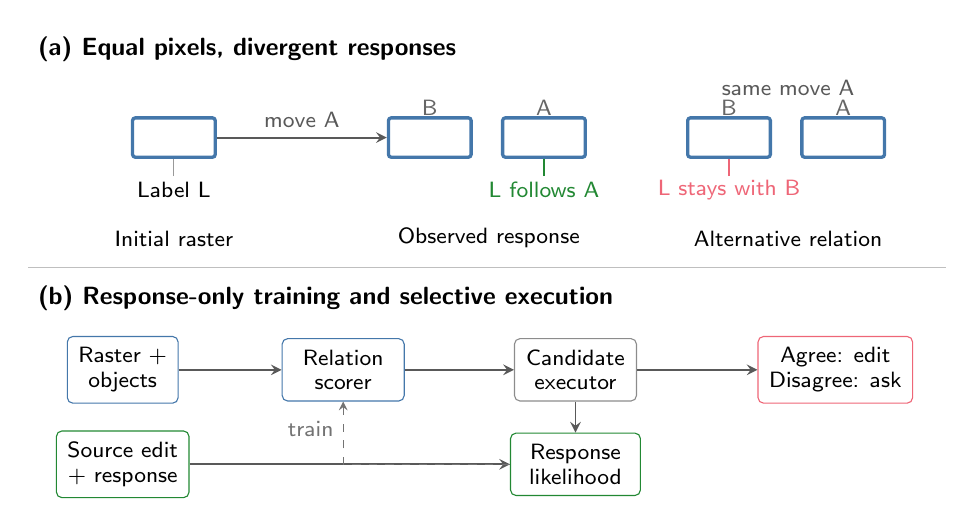
\begin{tikzpicture}[x=1cm,y=1cm,>=stealth,
  textstyle/.style={font=\sffamily\fontsize{8}{9}\selectfont},
  head/.style={font=\sffamily\fontsize{9}{10}\selectfont\bfseries},
  module/.style={draw=ptblue,very thick,rounded corners=1pt,minimum width=1.05cm,minimum height=.50cm,textstyle},
  nodebox/.style={draw=black!45,rounded corners=2pt,minimum height=.75cm,textstyle,align=center,inner sep=4pt},
  flow/.style={->,line width=.7pt,black!65}]
  \node[head,anchor=west] at (0,3.52) {(a) Equal pixels, divergent responses};
  \node[module] (a0) at (1.85,2.40) {};
  \node[textstyle] at (1.85,1.74) {Label L};
  \draw[black!40] (1.85,1.91) -- (1.85,2.13);
  \node[textstyle] at (1.85,1.12) {Initial raster};
  \node[module] (b1) at (5.1,2.40) {};
  \node[module] (a1) at (6.55,2.40) {};
  \node[textstyle,text=black!60] at (5.1,2.78) {B};
  \node[textstyle,text=black!60] at (6.55,2.78) {A};
  \draw[flow] (a0.east) -- node[above,textstyle] {move A} (b1.west);
  \node[textstyle,text=ptgreen] at (6.55,1.74) {L follows A};
  \draw[ptgreen,line width=.65pt] (6.55,1.91) -- (6.55,2.13);
  \node[textstyle] at (5.85,1.12) {Observed response};
  \node[textstyle,text=black!65] at (9.65,3.03) {same move A};
  \node[module] at (8.9,2.40) {};
  \node[module] at (10.35,2.40) {};
  \node[textstyle,text=black!60] at (8.9,2.78) {B};
  \node[textstyle,text=black!60] at (10.35,2.78) {A};
  \node[textstyle,text=ptred] at (8.9,1.74) {L stays with B};
  \draw[ptred,line width=.65pt] (8.9,1.91) -- (8.9,2.13);
  \node[textstyle] at (9.65,1.12) {Alternative relation};
  \draw[black!25] (0,.75) -- (11.65,.75);
  \node[head,anchor=west] at (0,.36) {(b) Response-only training and selective execution};
  \node[nodebox,draw=ptblue] (input) at (1.2,-.55) {Raster +\\ objects};
  \node[nodebox,draw=ptgreen] (source) at (1.2,-1.75) {Source edit\\ + response};
  \node[nodebox,draw=ptblue,minimum width=1.55cm] (score) at (4.0,-.55) {Relation\\ scorer};
  \node[nodebox,minimum width=1.55cm] (execute) at (6.95,-.55) {Candidate\\ executor};
  \node[nodebox,draw=ptgreen,minimum width=1.65cm] (loss) at (6.95,-1.75) {Response\\ likelihood};
  \node[nodebox,draw=ptred,minimum width=1.75cm] (decision) at (10.25,-.55) {Agree: edit\\ Disagree: ask};
  \draw[flow] (input) -- (score);
  \draw[flow] (score) -- (execute);
  \draw[flow] (execute) -- (decision);
  \draw[flow] (source) -- (loss);
  \draw[flow] (execute) -- (loss);
  \draw[->,dashed,black!55] (loss.west) -| node[pos=.78,left,textstyle] {train} (score.south);
\end{tikzpicture}

\caption{Equal initial pixels can lead to different edited states. In (a), hidden modules A and B share the left box; their letter IDs are schematic annotations, not rendered text. Moving A yields one of two label locations. In (b), source edits supervise latent relations, while test-time agreement covers only retained candidates.}
\label{fig:response}
\end{figure*}

Recent work already treats editability as a structural objective. VectorHarness recovers native authoring objects and operational relations, evaluates relation-preserving edits, and repairs affected regions \citep{tang2026vectorharness}. Back2Struct recovers object-level Scalable Vector Graphics (SVG) with text, shapes, topology, and layout \citep{yan2026back2struct}. ReFigBench evaluates editable PowerPoint reconstruction on real overview figures \citep{fan2026refigbench}. Typed graphs, local repair, and editable reconstruction therefore cannot define our research delta.

The training question concerns how to learn these dependencies without drawing relation-edge labels for every figure. Author-observed before/after edits give weaker, task-relevant supervision: candidate relations that predict the observed state receive probability mass. At test time, a requested edit may expose disagreement among visually plausible candidates, as Figure~\ref{fig:response} shows. The edit treats distinct graphs with identical responses as equivalent. Decision-focused abstractions already use task-relevant targets \citep{poli2023ideal}; latent graph inference from observed dynamics also has a long precedent \citep{kipf2018nri}.

The proposed pipeline has three stages: primitive extraction, candidate scoring, and selective execution. Perceptual tools extract boxes, text, and connector geometry. A small scorer ranks possible dependencies from the initial image without seeing the requested edit. A deterministic executor maps each candidate to a response and updates the dependency closure, the edited modules and their descendants. Training uses responses recorded from executable authoring sources, not responses simulated from a guessed relation. This division lets experiments isolate relation learning from optical character recognition and shape detection.

This draft contributes a precise learning problem, a response-only objective, and two scoped mathematical results: initial-render ambiguity and conditional local preservation. The objective remains untrained. The planned study must test whether response-only learning improves edited-state accuracy against equal-input baselines and whether selective execution reduces wrong edits at useful coverage. The browser converter supplies engineering infrastructure, not evidence for these learning claims.

\section{Prior work defines the boundary}
\paragraph{Reconstruction and vector generation.}
StarVector generates vector-graphics code from image tokens \citep{rodriguez2025starvector}; OmniSVG uses a structured token representation \citep{yang2025omnisvg}. LIVE optimizes paths through differentiable rendering \citep{ma2022live}. SliDer reconstructs document elements and refines the output \citep{hazimeh2026slider}. Back2Struct reconstructs object-level SVG from structured images and evaluates rendering, structural content, and directed flow \citep{yan2026back2struct}. Its reported rubric checks whether arrows connect the intended nodes; it does not report responses to controlled module movements. These works supply reconstruction baselines and representations. We do not infer their edit-response accuracy from their reported rendering metrics.

\paragraph{Authoring and local updates.}
VectorHarness directly addresses relation-preserving scientific-graphic reconstruction \citep{tang2026vectorharness}. SciDiagramEdit learns edits from paper revisions \citep{sun2026scidiagramedit}; Edit2TikZ benchmarks instruction-guided figure edits with restoration and off-target preservation metrics \citep{zhang2026edit2tikz}. VCG-Bench evaluates structured diagram generation and editing in mxGraph \citep{su2026vcgbench}. AutoFigure-Edit targets editable scientific illustration generation \citep{lin2026autofigureedit}. These systems and benchmarks already establish relation-aware authoring, edit-pair learning, and off-target checks. Our proposed comparison focuses on latent relation learning from controlled source-edit responses without training edge labels, followed by selective decisions at matched human and computational cost. We have not established an advantage over these neighboring approaches.

\paragraph{Programs and constraints.}
Graphics-program inference combines perceptual prediction with program synthesis \citep{ellis2018graphics}. Neural Relational Inference learns latent interaction graphs from observed dynamics \citep{kipf2018nri}. Constraint Scalable Vector Graphics expresses dependent layout through constraints \citep{badros2001constraint}. ExBind diagnoses visual-to-executable reference selection \citep{wang2026exbind}. Our setting observes sparse module edits in diagrams rather than trajectories of physical objects; this difference requires a direct baseline comparison.

\paragraph{Abstention and prediction sets.}
Structured Output Learning with Abstention already permits partial rejection of structured labels \citep{garcia2018sola}. Reject-option learning also covers structured-output tasks \citep{franc2023reject}, and risk-controlling prediction sets calibrate set-valued outputs from held-out data \citep{bates2021rcps}. Decision-focused learning already studies abstractions that retain information relevant to downstream decisions \citep{poli2023ideal}. Active program synthesis can choose informative questions among consistent programs \citep{tiwari2020significant}. We treat these capabilities as existing tools. Our candidate combines response-supervised graph scoring with edit-conditioned selection. We will test whether it improves decisions beyond edge prediction and these selective baselines. A full audit of task-specific adaptations remains necessary.

\section{A render does not identify response}
\subsection{Objects and dependency rules}
An authoring program is a pair $(X,G)$: an evaluated object state $X$ and a dependency graph $G$. State $X$ stores uniquely identified objects, their geometry, styles, strings, and drawing order; it excludes dependency identities. A module has an axis-aligned box $(x,y,w,h)$ with $w,h>0$. A label has a string and an anchor. A connector has two endpoints. In the proposed learner, only modules can be parents; labels and connector endpoints are leaves. Each derived object has one rule that computes its geometry from module parents. This bipartite graph has no directed cycles.

A connector has one joint rule that evaluates both endpoint attachments, so its two anchors do not create multiple object writers. A label attached to module $m$ has fixed normalized offsets $(u,v)$ and anchor
\begin{equation}
 p_m(u,v)=(x_m+u w_m,\ y_m+v h_m).
\end{equation}
A connector endpoint uses the same function. Boundary attachments require $(u,v)$ to lie on the unit-square boundary. The rule stores object identities as well as coordinates. Label strings remain literal data during module translation and resizing.

Let $R(X)$ denote a fixed deterministic renderer that reads evaluated geometry, style, text, and drawing order, and ignores dependency identities. An edit $e=(T,\delta)$ changes the free geometry of target modules $T$. The operator $F_G(X,e)$ applies those changes and evaluates dependent rules, returning an evaluated object state. We define the numeric \emph{edit response} as
\begin{equation}
 D_G(X,e)=\operatorname{geom}(F_G(X,e))-\operatorname{geom}(X),
\end{equation}
where $\operatorname{geom}$ concatenates numeric fields in a fixed object order. Text preservation is a separate equality predicate on strings. The edit family contains translations and positive axis-aligned resizings. It excludes text reflow, arbitrary relayout, and graph rewrites.

\subsection{Coincident modules hide attachment}
\begin{proposition}[Initial-render ambiguity]
There exist programs $(X,G_A),(X,G_B)$ with the same initial render and different edit responses to the same module translation.
\end{proposition}
\begin{proof}
Place two identically styled modules $A$ and $B$ at the same box in $X$. Place label $L$ at the shared center. In $G_A$, attach $L$ to $A$; in $G_B$, attach it to $B$. Both graphs evaluate to $X$, and $R$ reads only $X$, so their initial renders agree. Translate only $A$ by a nonzero vector $d$. The label moves by $d$ under $F_{G_A}$ and stays fixed under $F_{G_B}$. The two responses differ.
\end{proof}

The construction establishes an existence result. It does not estimate how often ambiguity occurs in scientific figures. A deterministic raster-only estimator returns the same answer for these identical inputs and therefore cannot match both hidden authoring states. Sampling or a learned prior can prefer one state, but the initial image supplies no evidence that distinguishes this pair.

\begin{definition}[Edit-conditioned response class]
Fix an evaluated state $X$ and a set of allowed edits $E$. Among graphs compatible with $X$, write $G\sim_{X,E}H$ when $F_G(X,e)$ and $F_H(X,e)$ have identical evaluated object states for every $e\in E$. For a single requested edit, $E=\{e\}$. This equality defines an equivalence relation on compatible graphs.
\end{definition}

The counterexample graphs lie in different classes when $E$ contains a translation of $A$. Add an unrelated module $C$ to both programs and let $E$ contain only a translation of $C$; the graphs then lie in the same class. Thus graph identity can be stricter than correctness for a requested edit. This observation motivates response-level training and evaluation, but an equivalence relation alone is not a learning contribution. Source edit behavior or author confirmation must identify the intended class when the input raster leaves it ambiguous.

\section{Observed edits constrain latent relations}
\subsection{Candidate rules preserve the initial state}
Primitive extraction supplies object boxes, recognized strings, and connector endpoints. For each label or endpoint, candidate scoring retains nearby module identities and a null attachment. An attached anchor initially at $(a_x,a_y)$ gets offsets $u=(a_x-x_m)/w_m$ and $v=(a_y-y_m)/h_m$. A boundary endpoint is compatible only when these offsets lie on the unit-square boundary; the formal model rejects other boundary candidates rather than projecting the anchor. A label may have any finite offsets. A null rule preserves the anchor's initial coordinates. Thus every retained rule evaluates to the same initial $X$. Detector noise and approximate boundary snapping require a separate initialization protocol and evaluation; the formal statements below concern exact compatible states.

A geometry baseline scores normalized boundary distance and overlap. The proposed learner uses a two-layer multilayer perceptron over relative position, relative size, endpoint direction, and text-box alignment. We have not trained this model.

One planned instantiation assigns a logit to each compatible parent/null choice. A graph score sums its selected choice logits. Beam search retains at most $K$ partial assignments, then assembles each connector's endpoint choices into one joint rule. The final beam contains complete bipartite graphs with one writer per derived object. It stores original text strings independently of geometry. Candidate truncation can omit the intended behavior, so agreement within this set never establishes candidate completeness.

\subsection{Marginal likelihood needs no edge labels}
Let $I$ denote the initial raster and detected objects. A source figure supplies edits $e_1,\ldots,e_T$ and observed edited object states $Y_1,\ldots,Y_T$ with stable object and connector-endpoint identities. A native source may encode relations, but the training loader hides that metadata. It exposes only the raster, object geometry and strings, edit commands, and resulting states. We claim no annotation-cost saving before measuring source preparation effort. Let $\mathcal R_j(I)$ contain the compatible attachment choices for label or endpoint $j$, including a free-anchor choice. The scorer predicts $q_\theta(r\mid I,j)$ without observing a future test edit. A fixed executor maps a choice and source edit to a predicted state $F_r(X,e_t)_j$.

The proposed loss marginalizes choices that explain the same source responses:
\begin{align}
\mathcal L_{\mathrm{resp}}(\theta)
 &=-\sum_j\log\sum_{r\in\mathcal R_j(I)}
 q_\theta(r\mid I,j)\,\Lambda_j(r),
\label{eq:response-loss}\\
\Lambda_j(r)
 &=\prod_{t=1}^{T}p_\sigma\left(Y_{t,j}\mid F_r(X,e_t)_j\right),
\end{align}
where $p_\sigma$ scores normalized coordinate error under a fixed observation-noise scale. We would choose that scale on a development split, then freeze it. Missing strings, inventories, object correspondences, or endpoint identities invalidate the local likelihood; we record such cases and measure them in end-to-end evaluation. The local product assumes conditional independence across observed edits for a fixed choice. Joint connector geometry follows the pair of inferred endpoint choices. Beam membership remains discrete; gradients flow through retained logits.

The loss learns an \emph{edit-response class}, not necessarily a unique graph. If two candidates produce identical states for every observed edit, their likelihood terms match and the data cannot separate their scores. An intervention on a module where their predictions diverge supplies the missing information. This identifiability limit motivates diverse training edits and explicit test-time disagreement. It also forbids treating a self-simulated edit as a new training label: external source behavior or author confirmation must supply $Y$.

We will compare marginal response learning with geometry rules, response-derived hard pseudo-edge labels, and a direct coordinate-response regressor under the same initial objects and training edits. Fully annotated edges form an additional-information upper bound, not the primary comparator. The requested edit enters the executor and selection rule below; an edit-conditioned scorer is a separate ablation. No supervised edge term appears in Equation~\ref{eq:response-loss}.

\subsection{Agreement permits bounded decisions}
Selective execution compares the retained graphs under a requested edit. Define
\begin{align}
 Z_G(X,e)&=N\operatorname{geom}(F_G(X,e)),\\
 a(\mathcal C,X,e)&=\max_{G,H\in\mathcal C}\|Z_G(X,e)-Z_H(X,e)\|_\infty,
\end{align}
where $N$ normalizes coordinate fields by the initial canvas width or height as above. An empty candidate set forces abstention before computing the maximum. Different object inventories or label strings also force abstention. For a tolerance $\tau\geq0$, the executor accepts only when $a\leq\tau$ and executes the highest-scoring retained graph, breaking ties by a fixed ordering. In unassisted mode, a failed agreement check ends in abstention. In assisted mode, it may trigger an attachment query that separates disagreeing graphs. A confirmed relation removes inconsistent candidates, and the executor repeats the check; an empty set after confirmation forces abstention. The query policy and burden remain unmeasured.

If the candidate set contains the intended graph, an accepted output differs from its normalized numeric response by at most $\tau$. This follows because the selected and intended graphs form one pair in the maximum. This bound guarantees exact numeric response correctness when $\tau=0$. If the intended graph lies outside the set, agreement can give a wrong answer. We call this decision \emph{conditional agreement within tolerance}, not an unconditional guarantee of author intent. Statistical confidence requires an independent calibration protocol that includes candidate omissions.

\subsection{Closure restricts state changes}
The dependency closure $C_G(T)$ contains edited modules and every graph descendant. The executor changes free target geometry, visits derived objects in topological order, and recomputes only objects in this closure. It preserves all other object fields.

\begin{proposition}[Conditional local preservation]
Assume a consistent initial state, an acyclic graph, one writer per derived object, and an edit from the specified family that leaves all dimensions positive. Closure propagation preserves every label/attachment equation. Objects outside $C_G(T)$ have identical states before and after the edit. Label strings remain unchanged.
\end{proposition}
\begin{proof}
An object outside the closure has no edited ancestor. The executor never assigns its fields, so its state stays identical. For a derived object inside the closure, every parent precedes it in topological order. Re-evaluating its rule therefore uses the updated parent states and satisfies its defining equation. Induction over this order proves the claim for every affected derived object. Rules assign geometry only, so they preserve strings.
\end{proof}

The property depends on supplied rules. It does not prove that a predicted graph captures the intended dependency. It also concerns object state, not unchanged pixels: moving an object can change occlusion outside its original footprint. Font rendering, export compilation, and connector routing need separate checks. The current JavaScript prototype implements single-target edits, label anchors, straight connectors, and candidate disagreement. It does not infer any of them from pixels.

\section{Source edits must test the claim}
\begin{table*}[t]
\caption{Planned comparison matrix. Each row names a needed experiment, not a reported result. All comparisons use independent source-figure splits.}
\label{tab:plan}
\centering\small
\renewcommand{\arraystretch}{1.25}
\begin{tabular}{@{}p{.18\textwidth}p{.47\textwidth}p{.26\textwidth}@{}}
\toprule
Test & Matched comparison & Primary measures \\
\midrule
Response learning & Geometry; response-derived hard labels; direct response regression; marginal response learning & Edited-state accuracy; candidate omission \\
\addlinespace[3pt]
Selective editing & Agreement; score rejection; larger beam; random, edge-entropy, and always-ask queries & Risk at matched coverage and human time \\
\addlinespace[3pt]
End-to-end recovery & Reference versus detected primitives; runnable vector and native-authoring systems & Text and endpoint accuracy; raster fallback; runtime and memory \\
\bottomrule
\end{tabular}
\end{table*}
\subsection{Source figures define independent units}
The primary training subset needs licensed authoring sources with persistent object and endpoint IDs, raster exports, specified edits, and observed edited states. A native source or author may execute each controlled edit; the training loader reads resulting states but masks source relation metadata. A static SVG supplies objects and visible arrows but may omit operational rules. Static exports alone cannot establish response ground truth. A separate evaluation subset may use author-confirmed before/after edits with verified object and endpoint correspondence. Reversed or rerouted connectors require explicit endpoint tracking; otherwise we exclude that edit from local likelihood and count it as a full-pipeline failure. We will split original sources and template families before generating variants. Repeated edits of one figure remain dependent measurements.

Each method will process the same figure/edit pairs. We will randomize run order within source-figure blocks and record provider versions, seeds, detector configuration, and resource limits. Annotation and scoring will hide method identities. Mechanism comparisons will hold primitives, optical character recognition, and human-query budget fixed. Full-pipeline comparisons will retain each method's documented configuration and report its resource cost.

\subsection{Named baselines test distinct claims}
The first comparison uses nearest-boundary geometry, response-derived hard pseudo-edge labels with logistic regression or XGBoost, a matched-capacity hard-label multilayer perceptron, and the marginal response learner. A direct per-object regressor predicts edited label anchors and connector endpoints from the same primitives and edit specification. These controls test whether latent marginalization adds value beyond geometry, hard labels, and direct response prediction. A fully edge-supervised model receives extra information and serves only as an upper bound. Edit-conditioned scoring is an ablation against the edit-independent scorer.

End-to-end comparisons will include available StarVector, OmniSVG, LIVE, and Image-to-PPT \citep{sun2026imageppt} implementations. Back2Struct and VectorHarness are closer comparisons for native objects and editable relations; we must use runnable releases or clearly label any missing executable baseline. ReFigBench, Edit2TikZ, and VCG-Bench supply task and metric precedents, but their distinct input, output, and edit protocols prevent direct score transfer. We will adapt a source-paired controlled-edit subset and compare runnable methods under one protocol. The inspected VectorHarness repository contains a brief README, and SliDer marks implementation release as forthcoming. Their paper-reported values will not substitute for controlled runs.

Query experiments will compare disagreement-driven confirmation with random, edge-entropy, and always-ask policies at the same fixed answer budget. Ordinary score rejection and a larger candidate beam test whether the proposed decision rule adds value. Unassisted risk-versus-coverage curves disable queries. Assisted curves report coverage and executed-edit risk for each fixed answer budget, together with human time. Interactive and unassisted methods will not share an unqualified score.

\subsection{Metrics expose correctness and cost}
Text accuracy compares source and recovered strings before and after edits. On the separately edge-annotated audit subset, attachment preservation measures whether endpoints satisfy the independently specified parent boundary rule, and outside-closure state drift measures numeric changes to objects with no intended dependency on the target. These two structural measures are undefined for the remaining figures: edited states alone do not reveal the intended parent or its closure. An independently annotated edit-footprint subset supports a separate off-target pixel-change measure, including occlusion. Raster fallback area records how much content remains uneditable.

Mechanism tests with reference primitives use exact state equality to measure whether the candidate set contains the intended edit-response class. Full-pipeline tests require independently verified mapping between recovered and source objects. A missing or extra object, an incorrect label string, or a wrong source-to-output mapping counts as a wrong edited response. For aligned objects, numeric edited-state error uses the normalized maximum coordinate difference; a response counts as correct only when that error stays at most a fixed evaluation tolerance $\epsilon$. We will set $\epsilon$ from development-set annotation resolution before inspecting held-out outcomes. It differs from the acceptance threshold $\tau$, which controls coverage. We will audit source attachment identity only in the separately annotated subset: a graph may respond correctly to one edit while storing a wrong relation for a later edit. Full-pipeline comparisons on the larger response-paired set use object-state error and text accuracy, not unobservable relation or closure labels.

Unassisted risk-versus-coverage curves report the fraction of wrong responses among executed edits as $\tau$ varies. Edit-response recall measures whether any retained graph matches the reference edited state exactly in mechanism tests or within $\epsilon$ in full-pipeline tests. An edge-annotated audit subset will measure graph recall and the rate at which a wrong graph still gives the correct requested response. Candidate omission remains in every denominator for recall and coverage; an executed edit with omitted truth remains in selective risk. We will disaggregate by endpoint ambiguity, overlap, graph size, text length, and unseen source family. End-to-end latency and peak memory include perception, scoring, search, execution, and export.

\subsection{Failure criteria govern continuation}
The study will compare variants that replace marginalization with hard response-derived labels, restrict candidate diversity, or remove abstention. If geometry or hard labels match the learner, agreement fails on unseen source families, or a larger beam plus ordinary rejection matches the risk-cost curve, the proposed learning contribution needs revision. Low response-class recall or a negligible ambiguity rate in representative figures would also weaken the motivation. A conditional proof and a toy example alone do not establish a conference-level contribution.

We have run only prototype software checks and engineering conversion tests. Table~\ref{tab:plan} maps claims to the comparisons that could test them; it contains no outcomes. We will choose an independent-source sample size after a pilot estimates variability. This draft does not claim a representative population result.

\section{Scope and next decision}
Selective edit-response recovery is a candidate research question about decisions under uncertain dependencies. The mathematical construction establishes that an initial render can underdetermine edit response, while the executor proof supplies a bounded preservation property given correct rules. Neither result establishes learning performance or originality against all neighboring work.

The scope excludes arbitrary illustrations, nonlinear chart semantics, text reflow, cyclic constraints, and cross-format preservation. A small relation head may still depend on costly perception. Omitted graphs can defeat agreement; human confirmation adds work. Source-paired evidence must separate these costs from benefits.

\section*{Impact statement}
Recovering editable scientific figures can reduce manual redrawing, but an incorrect dependency or label can change scientific meaning. Tools should retain the original, record accepted edits, distinguish raster from native objects, and require comparison before publication. Source-program data and reproduced figures require suitable licenses and author permission. Users should keep confidential manuscripts local unless an approved provider policy permits transmission.

\begingroup
\small
\balance
\bibliography{references}
\bibliographystyle{style/icml2026}
\endgroup
\end{document}
